\large



The study found that the GWPL was the best method to predict the PL, however the value of the surface constant was needed to be complex and therefore hard to determine. The accuracy of the models was found to:

\begin{center}
\begin{tabular}{|c|c|c|}
\hline
\textbf{Models} & \textbf{MSE} & \textbf{Applicability} \\ \hline
FSPL            & 15.95        & 35 \%                  \\ \hline
ATRPL 		    & 141.58       & 65 \%                  \\ \hline %approx.
%TRPL     		& 42.12        & 100 \%                 \\ \hline
GWPL            & 35.49        & 100 \%                 \\ \hline
NSPL            & 230.05       & 30 \%                  \\ \hline
NPPL            & 60.18        & 65 \%                  \\ \hline
\end{tabular}
\end{center}


In the study it was found that the value of the surface constants, gave rise to a offset in the PL. This constant is however not easy to accurately determine. 
% This file was created by matlab2tikz.
%
%The latest updates can be retrieved from
%  http://www.mathworks.com/matlabcentral/fileexchange/22022-matlab2tikz-matlab2tikz
%where you can also make suggestions and rate matlab2tikz.
%
\definecolor{mycolor1}{rgb}{0.00000,0.44700,0.74100}%
\definecolor{mycolor2}{rgb}{0.85000,0.32500,0.09800}%
\definecolor{mycolor3}{rgb}{0.92900,0.69400,0.12500}%
%
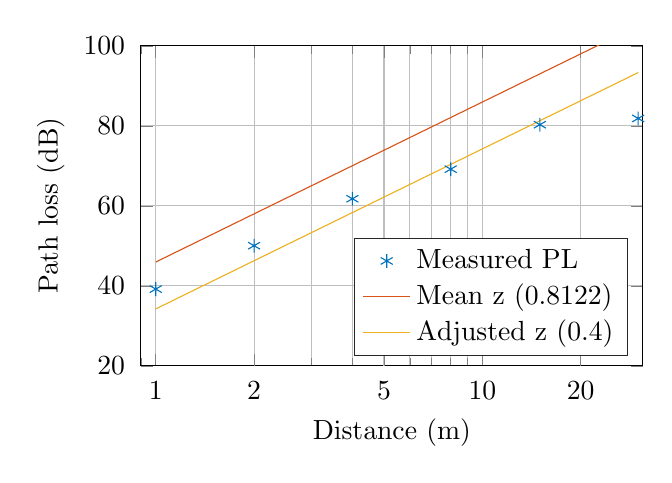
\begin{tikzpicture}

\begin{axis}[%
width=2.51in,
height=1.6in,
at={(2.6in,1in)},
scale only axis,
extra x ticks={2,5,20}, 
extra x tick style={log identify minor tick positions=false},
log ticks with fixed point,
xticklabel style={yshift=-0.5ex},
yticklabel style={xshift=-0.5ex},
xmode=log,
xmin=0.9,
xmax=31,
xlabel=Distance (m),
xminorticks=true,
xmajorgrids,
xminorgrids,
ymin=20,
ymax=100,
ylabel=Path loss (dB),
ymajorgrids,
axis background/.style={fill=white},
legend style={at={(0.03,0.97)},anchor=north west,legend cell align=left,align=left,draw=white!15!black},
legend pos = south east
]
\addplot [color=mycolor1,mark size=2.5pt,only marks,mark=asterisk,mark options={solid}]
  table[row sep=crcr]{%
1	39.176832441447\\
2	50.0236813268286\\
4	61.7627349006033\\
8	69.1568155321866\\
15	80.2784721484843\\
30	81.8463231335614\\
};
\addlegendentry{Measured PL};

\addplot [color=mycolor2,solid]
  table[row sep=crcr]{%
1	45.9420286016976\\
2	57.9832284282568\\
4	70.0244282548161\\
8	82.0656280813753\\
15	92.9856789639248\\
30	105.026878790484\\
};
\addlegendentry{Mean z (0.8122)};

\addplot [color=mycolor3,solid]
  table[row sep=crcr]{%
1	34.2247802230071\\
2	46.2659800495663\\
4	58.3071798761256\\
8	70.3483797026848\\
15	81.2684305852343\\
30	93.3096304117936\\
};
\addlegendentry{Adjusted z (0.4)};

\end{axis}
\end{tikzpicture}%
